\documentclass[11pt,italian]{article}
\usepackage[T1]{fontenc}
\usepackage[utf8]{inputenc} %utf8 % lettere accentate da tastiera
\usepackage[italian]{babel} % lingua del documento
\usepackage{blindtext}
\usepackage{enumitem}
\usepackage{graphicx}
\usepackage{float}
\usepackage{xcolor}   % for \textcolor
\usepackage[font=small,labelfont=bf,skip=3pt]{caption}
\setlength{\belowcaptionskip}{-10pt}
\usepackage{listings}
\lstset{
    basicstyle=\small\ttfamily,
    columns=fullflexible,
    frame=single,
    breaklines=true,
    postbreak=\mbox{\textcolor{red}{$\hookrightarrow$}\space},
    tabsize=4, % tab space width
    showstringspaces=false, % don't mark spaces in strings
    numbers=left, % display line numbers on the left
    commentstyle=\color[HTML]{a0a1a7}, % comment color
    keywordstyle=\color[HTML]{40a3f5}, % keyword color
    stringstyle=\color{red}, % string color,
    emphstyle={\color[HTML]{40a3f5}}
}

\usepackage{hyperref}
\usepackage{cleveref}
\hypersetup{
    colorlinks = true,
    linkbordercolor = {white},
    urlcolor = blue
}
\usepackage{graphicx}
\graphicspath{ {./images/} }

% Italian syntax spacing
\frenchspacing

% Line height
\renewcommand{\baselinestretch}{1.15}

\title{
    Metodi del Calcolo Scientifico \\
    \normalsize Progetto 1 \\
    \normalsize Risoluzione di sistemi lineari tramite il metodo di Cholesky \\
}

\date{\small A.A. 2019/2020}

\author{
    \normalsize
    \textsc{Edoardo Silva} 816560 \\
    \normalsize
    \textsc{Bryan Zhigui} 816335 \\
    \normalsize
    \textsc{Davide Marchetti} 815990
}

\begin{document}

\maketitle

\section*{Abstract}
Questo progetto si prefigge lo scopo di studiare l'implementazione del metodo di Choleski per la risoluzione sistemi lineari per matrici simmetriche definite positive sparse in un ambiente di programmazione open source e di compararli con l'implementazione closed-source di MATLAB.

Il confronto avverrà in termini di tempo, accuratezza, impiego della memoria e anche facilità d'uso sia in ambiente Linux che Windows, eseguendo il codice su diverse matrici derivate da problemi reali e raccolte nella \textbf{SuiteSparse Matrix Collection}\footnote{\url{https://sparse.tamu.edu/}}.

\newpage
\section{Analisi dell'implementazione}

\subsection{MATLAB}
Per la decomposizione di cholesky, MATLAB mette a disposizione il modulo \lstinline{Symbolic Math Toolkit} contenente tutto il necessario. In particolare è stata utilizzata la funzione \lstinline{chol}\footnote{\url{https://www.mathworks.com/help/matlab/ref/chol.html}}.

\subsubsection*{Utilizzo}
\lstinline{R = chol(A, [triangle])}: fattorizza la matrice $A$ simmetrica definita positiva in una matrice triangolare superiore $R$ tale che $A=R^{-1}R$.

Il parametro \lstinline{triangle} permette di scegliere se attuare la decomposizione in una matrice triangolare superiore (default) o triangolare inferiore.
In quest'ultimo caso, la matrice $R$ risultante dall'equazione soddisferà l'uguaglianza $A = RR^{-1}$.

\subsubsection*{Manutenzione}
La libreria è stata rilasciata per la prima volta nell'aggiornamento R2013a MATLAB. Attualmente, è ancora supportata e non presenta lacune o problemi riscontrati durante il suo utilizzo.

\subsubsection*{Documentazione}
La documentazione ufficiale di MATLAB è ben strutturata e di facile consultazione. Vengono anche proposti molti esempi di utilizzo delle diverse funzioni in varie casistiche.

\subsubsection*{Licenza}
Essendo MATLAB un software closed-source, non è possibile accedere al codice sorgente del modulo.

\subsubsection*{Problemi riscontrati}
La criticità principale riguarda il supporto del modulo \lstinline{memory} esclusivamente per sistemi operativi Windows. Difatti, è stato necessario utilizzare due metodi di profiling della memoria diversi a seconda del sistema operativo di esecuzione.

\subsection{Open-Source (C++)}
Dopo un'attenta analisi e comparazione di diverse opzioni, l'implementazione in C++ è stata costruita utilizzando \textbf{Eigen},  libreria che si pone l'obiettivo di essere leggera ed offrire supporto alle operazioni su vettori e matrici dense e sparse.

\subsubsection*{Utilizzo}
\lstinline{Eigen::loadMarket(A, filename)}: importa i valori di una matrice sparsa memorizzata in un file \lstinline{.mtx} nella matrice fornita come primo argomento. Nel nostro programma, \lstinline{A} è definita come \lstinline{Eigen::SparseMatrix<double>}.

Il modulo \lstinline{unsupported/Eigen/SparseExtra} che contiene queste funzionalità è attualmente deprecato.

\subsubsection*{Manutenzione}
Eigen è in sviluppo attivo, tuttavia, alcuni moduli sono marcati come deprecati e non ne è garantito il loro pieno funzionamento. Un esempio di questi è la classe \lstinline{MarketIO}, che permette di effettuare operazioni di input e ouput con file in formato \lstinline{Matrix Market (.mtx)}.

\subsubsection*{Documentazione}
La documentazione di Eigen è di facile consulto e abbastanza completa. Tuttavia, non si può fare la stessa considerazione rispetto ai moduli inseriti nel namespace \lstinline{unsupported}, per i quali la documentazione è spesso mancante o riferita a versioni precedenti.

\subsubsection*{Licenza}
Eigen è un software gratuito ed open-source rilasciato con licenza Mozilla Public License 2.0 (MPL2: simple weak copyleft license) dalla versione 3.1.1.

\subsubsection*{Problemi riscontrati}
L'utilizzo di una classe deprecata ha inizialmente rallentato lo sviluppo. Infatti, delle matrici importate tramite \lstinline{MarketIO} veniva ignorato il fatto che fossero salvate come simmetriche o meno.

Questo inconveniente è stato risolto modificando lo script di conversione MATLAB \lstinline{mmwrite} per trasformare file \lstinline{.mat} in \lstinline{.mtx} e rigenerando le matrici assicurandosi che tutti gli elementi venissero salvati correttamente.
Lo script utilizzato per la conversione è riportato nella \cref{section:code}.

Tuttavia, questa trasformazione aggiuntiva comporta uno spreco di spazio su disco per memorizzare il doppio dei valori rispetto ad un semplice indicatore che specifichi qualora la matrice sia simmetrica, e di tempo per la conversione dei file e per la lettura del doppio delle righe da file durante l'esecuzione.

\newpage
\section{Dettagli implementativi}
Riporteremo di seguito le sezioni semplificate delle parti principali di ciascun'implementazione.
Lo schema di entrambi gli algoritmi coincide, le differenze sono date dalle peculiarità del linguaggio utilizzato.

Entrambi gli algoritmi accettano in input come parametro il percorso del file da analizzare ed effettuano le seguenti operazioni:
\begin{enumerate}
    \item Carico la matrice $M$ dal file specificato in input
    \item Memorizzo l'occupazione attuale della memoria
    \item Creo la soluzione esatta $x_{es}$ come vettore di elementi con valore $1$ pari alla dimensione della matrice $M$
    \item Calcolo il vettore $b$ dei termini noti
    \item Applico la decomposizione di Cholesky con il metodo scelto fornendo in input la matrice $M$ e il vettore $b$ memorizzando il tempo di esecuzione ed ottenendo la soluzione approssimata $x_{ap}$
    \item Calcolo la memoria utilizzata subito dopo la risoluzione del sistema
    \item Calcolo l'errore relativo tra $x_{ap}$ e $x_{es}$
    \item Restituisco tutte le metriche registrate al chiamante che si occuperà della memorizzazione su file
\end{enumerate}

\subsection{MATLAB}
In particolare, MATLAB accetta in input un file che si assume essere una matrice memorizzata in formato \lstinline{.mat}. Questo permette di caricarla semplicemente tramite la funzione \lstinline{load}.

Il listato \ref{code:matlab-algo} riporta la procedura descritta in precedenza utilizzata nella nostra implementazione.

\newpage
\begin{lstlisting}[language=Matlab,emph={ones},caption=MATLAB: Algoritmo principale,label=code:matlab-algo]
function [rows, memory_delta, solve_time, error] = chol_solve(name)
    load(fullfile('', 'matrix_mat', name), "Problem");

    [user] = memory;
    proc_memory_start = user.MemUsedMATLAB;

    rows = size(Problem.A, 1);
    x_es = ones(rows, 1);
    b = Problem.A * x_es;

    tic;
    R = chol(Problem.A);
    x_ap = R \ (R' \ b);
    solve_time = toc;

    [user] = memory;
    memory_delta = user.MemUsedMATLAB - proc_memory_start;

    error = norm(x_ap - x_es) / norm(x_es);
end
\end{lstlisting}

\subsection{C++}
Nell'implementazione C++ per la funzione \lstinline{analyze_matrix} si è scelto di definire una \lstinline{struct} contenente tutti i campi che era necessario ottenere in output (listato \ref{code:cpp-struct}).

Questo permette di semplificare il codice evitando di utilizzare più parametri passati per indirizzo come valori di output.

\begin{lstlisting}[language=C++,emph={ull,std},caption=C++: Struct per la memorizzazione del risultato,label=code:cpp-struct]
typedef unsigned long long ull;
struct result {
    unsigned int size;
    ull memory_delta;
    std::chrono::duration<double> solve_time;
    double relative_error;
};
\end{lstlisting}

\noindent
L'implementazione del solutore ricalca gli step definiti precedentemente. La lettura della memoria utilizzata avviene utilizzando metodi di una classe personalizzata scritta ad-hoc per il progetto e riportata nella \cref{section:code}.
\begin{lstlisting}[language=C++,emph={result,SpMat,Eigen,int,std},caption=C++: Algoritmo principale,label=code:cpp-algo]
result analyze_matrix(std::string filename) {
    result r;
    SpMat A; // Eigen::SparseMatrix<double>
    ull start_mem, end_mem;

    Eigen::loadMarket(A, filename);
    r.size = A.rows();

    start_mem = memory::process_current_physical();

    Eigen::VectorXd x_es = Eigen::VectorXd::Ones(A.rows());
    Eigen::VectorXd b(A.rows());
    b = A*x_es;

    auto chol_start = std::chrono::high_resolution_clock::now();
    Eigen::SimplicialCholesky<SpMat> chol(A);
    Eigen::VectorXd x_ap = chol.solve(b);
    auto chol_finish = std::chrono::high_resolution_clock::now();

    end_mem = memory::process_current_physical();

    r.memory_delta = end_mem - start_mem;
    r.solve_time = chol_finish - chol_start;
    r.relative_error = (x_ap - x_es).norm() / x_es.norm();
}
\end{lstlisting}

\newpage
\section{Specifiche hardware}
La piattaforma utilizzata per la produzione dei risultati riportati nelle \cref{section-results-impl,section-results-os}, è composta come segue:
\begin{itemize}
    \item \textbf{CPU}: AMD Ryzen 5 3600 - 6 Core / 12 Threads - 3.60Ghz /4.20Ghz
    \item \textbf{RAM}: Crucial Ballistix DDR4-3000C15 2*8Gb (16Gb) a 3800MHz
    \item \textbf{HDD}: Western Digital Green 1TB HDD
    \item \textbf{GPU}: Sapphire RX 580 Pulse (8GB VRam)
\end{itemize}

\noindent
Il disco utilizzato per l'esecuzione in ambiente Windows è un \textbf{SSD Samsung 850 EVO (250Gb)}, mentre Linux è installato su un \textbf{NVMe Sabrent (256Gb)}.

\newpage
\section{Matrici analizzate}
L'analisi si è concentrata sulle seguenti matrici:

\begin{table}[h]
    \centering
    \begin{tabular}{|l|r|r|}
        \multicolumn{1}{c}{\textbf{Nome}} & \multicolumn{1}{c}{\textbf{Dimensione}} & \multicolumn{1}{c}{\textbf{NNZ}} \\ \hline
        ex15 & 6.867 & 98.671 \\
        shallow\_water1 & 81.920 & 327.680 \\
        cfd1 & 70.656 & 1.825.580 \\
        cfd2 & 123.440 & 3.085.406 \\
        parabolic\_fem & 525.825 & 3.674.625 \\
        apache2 & 715.176 & 4.817.870 \\
        G3\_circuit & 1.585.478 & 7.660.826 \\
        StocF-1465 & 1.465.137 & 21.005.389 \\
        Flan\_1565 & 1.564.794 & 114.165.372 \\ \hline
    \end{tabular}
    \caption{Matrici analizzate}
    \label{tab:matrix-list}
\end{table}

\newpage
\section{Risultati per sistema operativo}
\label{section-results-impl}

\subsection{Windows}
\subsubsection*{Tempo}
All'incremento delle dimensioni della matrice di input non si manifesta una crescita lineare né costante in termini di tempo.
Ciononostante, i tempi di esecuzione nell'implementazione in MATLAB risultano essere meno variabili rispetto alla controparte in C++.
\begin{figure}[H]
    \makebox[\textwidth][c]{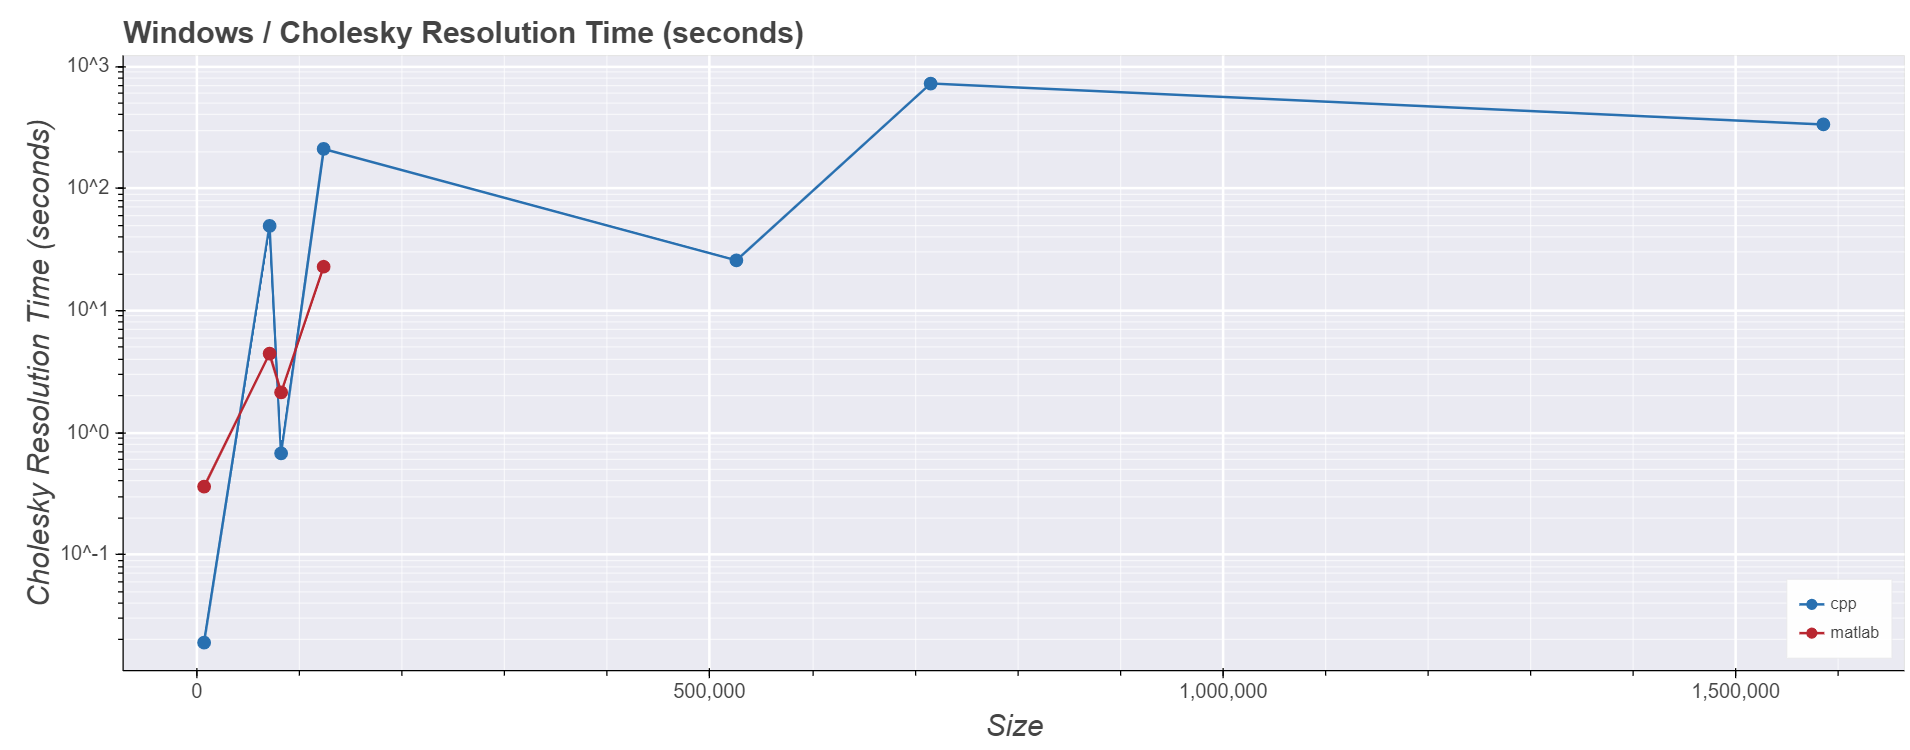
\includegraphics[width=1.3\linewidth]{windows_solve.png}}
    \caption{Tempo di risoluzione su Windows}
    \label{fig:windows-time}
\end{figure}

\smallskip
\subsubsection*{Memoria}
Come illustrato in \cref{fig:windows-memory}, l'implementazione in C++ occupa molta meno memoria rispetto a quella in MATLAB, in particolare al crescere della dimensione della matrice e del numero di elementi non nulli contenuti in essa.

Difatti, tutte le matrici analizzate in MATLAB per le quali non è presente un risultato nel grafico, durante la decomposizione di Cholesky hanno comportato un errore \lstinline{Out of memory}.
\begin{figure}[H]
    \makebox[\textwidth][c]{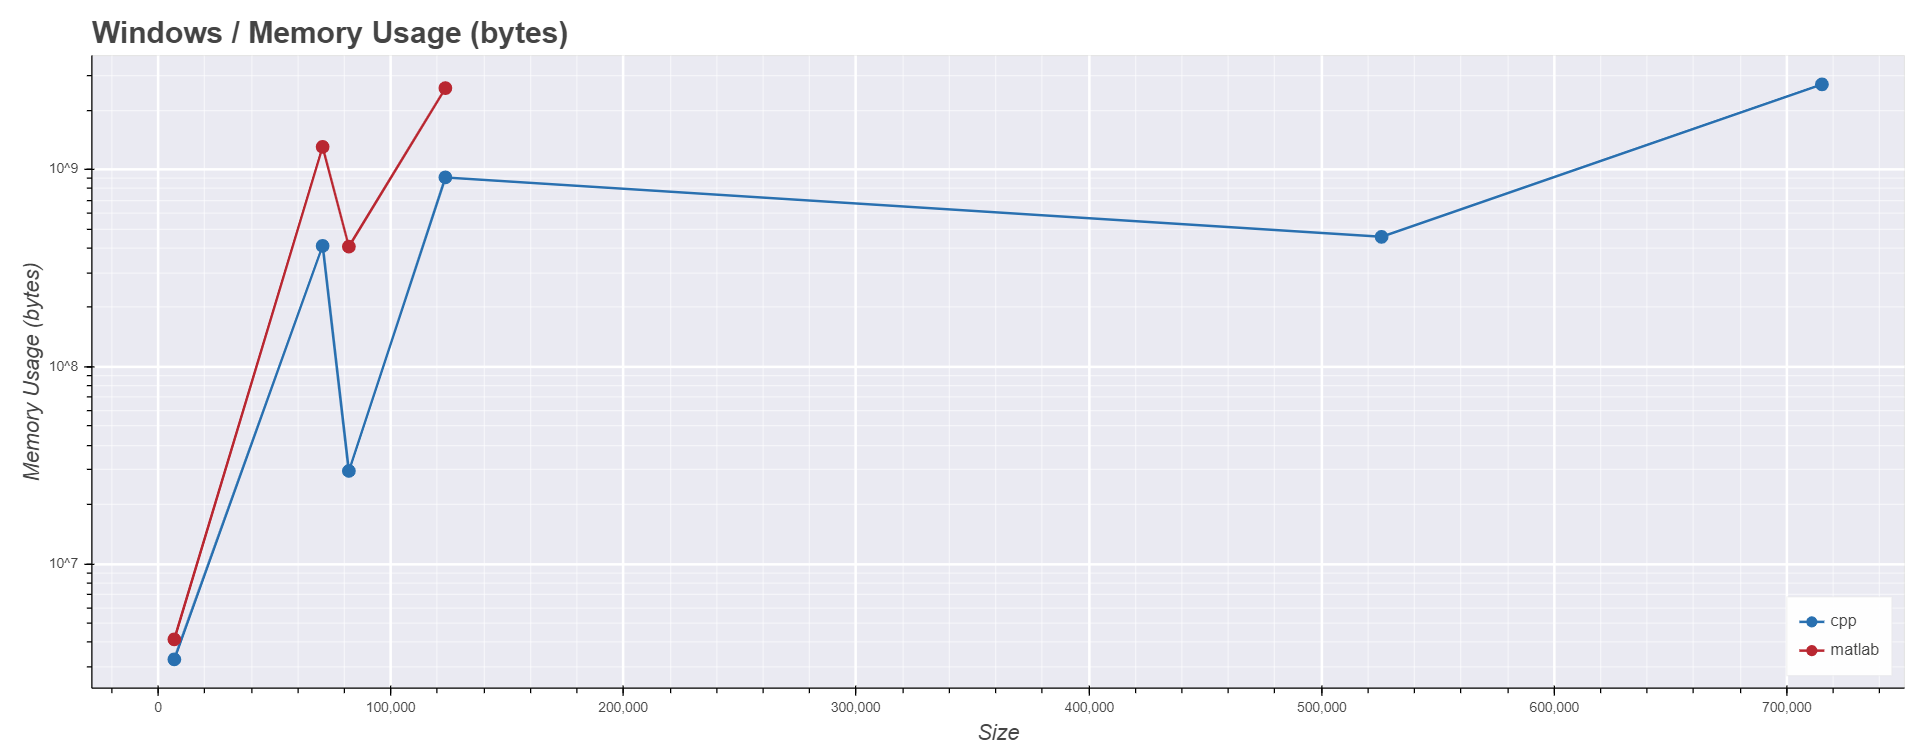
\includegraphics[width=1.3\linewidth]{windows_memory.png}}
    \caption{Utilizzo della memoria su Windows}
    \label{fig:windows-memory}
\end{figure}

\smallskip
\subsubsection*{Errore Relativo}
Entrambe le implementazioni presentano un errore relativo molto simile.
In \cref{fig:windows-error} si nota come al crescere della dimensione della matrice per C++ l'errore relativo sembra stabilizzarsi tra $10^{-10}$ e $10^{-12}$.
\begin{figure}[H]
    \makebox[\textwidth][c]{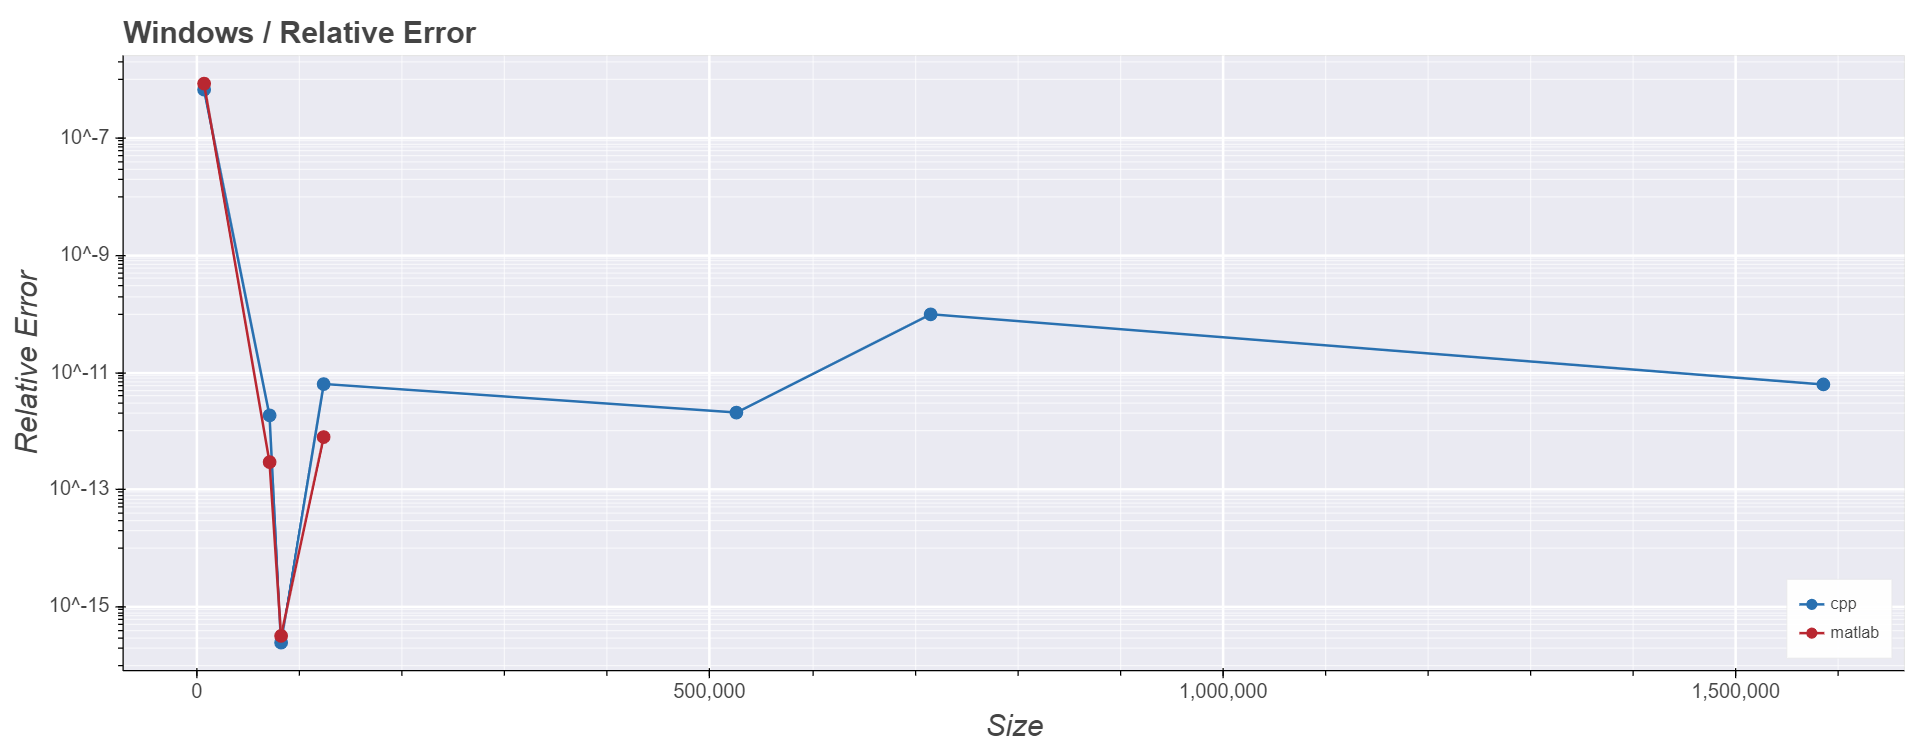
\includegraphics[width=1.3\linewidth]{windows_error.png}}
    \caption{Errore relativo su Windows}
    \label{fig:windows-error}
\end{figure}

\subsection{Linux}
\subsubsection*{Tempo}
L'andamento del tempo di risoluzione del sistema non risulta strettamente dipendente dalla dimensione della matrice. Inoltre, l'implementazione in MATLAB riesce a mantenere tempi di completamento meno variabili.
\begin{figure}[H]
    \makebox[\textwidth][c]{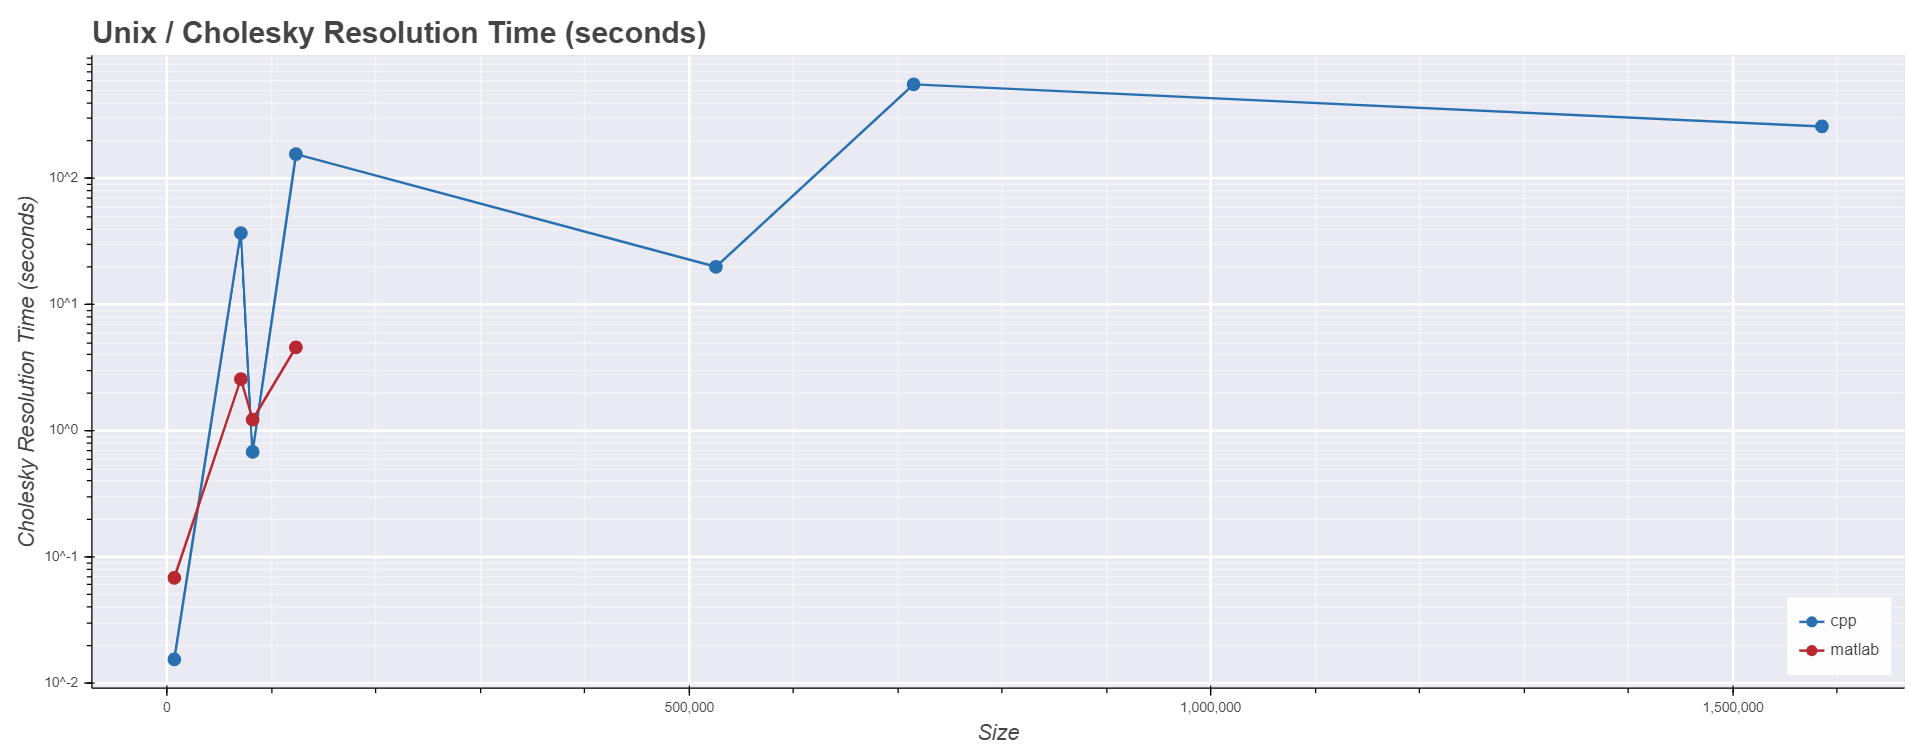
\includegraphics[width=1.2\linewidth]{unix_solve.png}}
    \caption{Tempo di risoluzione su Linux}
    \label{fig:linux-time}
\end{figure}

\subsubsection*{Memoria}
L'utilizzo della memoria, a differenza di quanto visto in precedenza nella \cref{fig:windows-memory} presenta una lettura iniziale molto bassa nell'implementazione MATLAB.
\begin{figure}[H]
    \makebox[\textwidth][c]{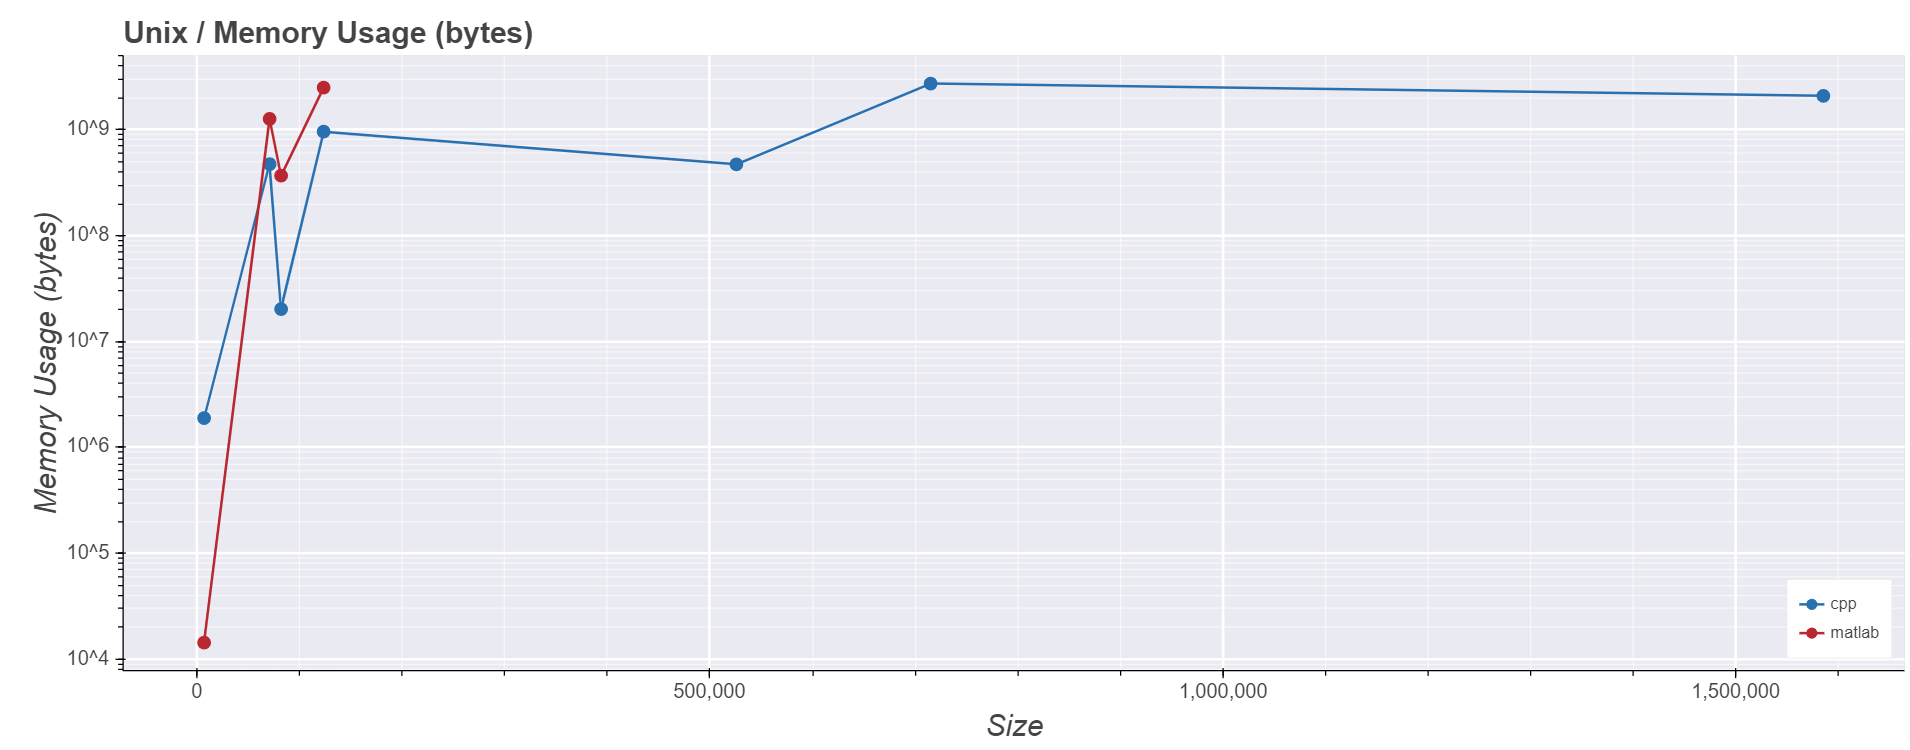
\includegraphics[width=1.2\linewidth]{unix_memory.png}}
    \caption{Utilizzo della memoria su Linux}
    \label{fig:linux-memory}
\end{figure}

\smallskip
\subsubsection*{Errore relativo}
Si nota che, sia su c++ che con la libreria MatLab, si ha un errore comparabile/quasi uguale per entrambi i metodi, e che dopo un massimo ed un minimo nelle matrici più piccole, l'errore si stabilizza intorno a $10^{-11}$, indipendentemente dalle dimensioni delle matrici che il programma riesce a caricare.
\begin{figure}[H]
    \makebox[\textwidth][c]{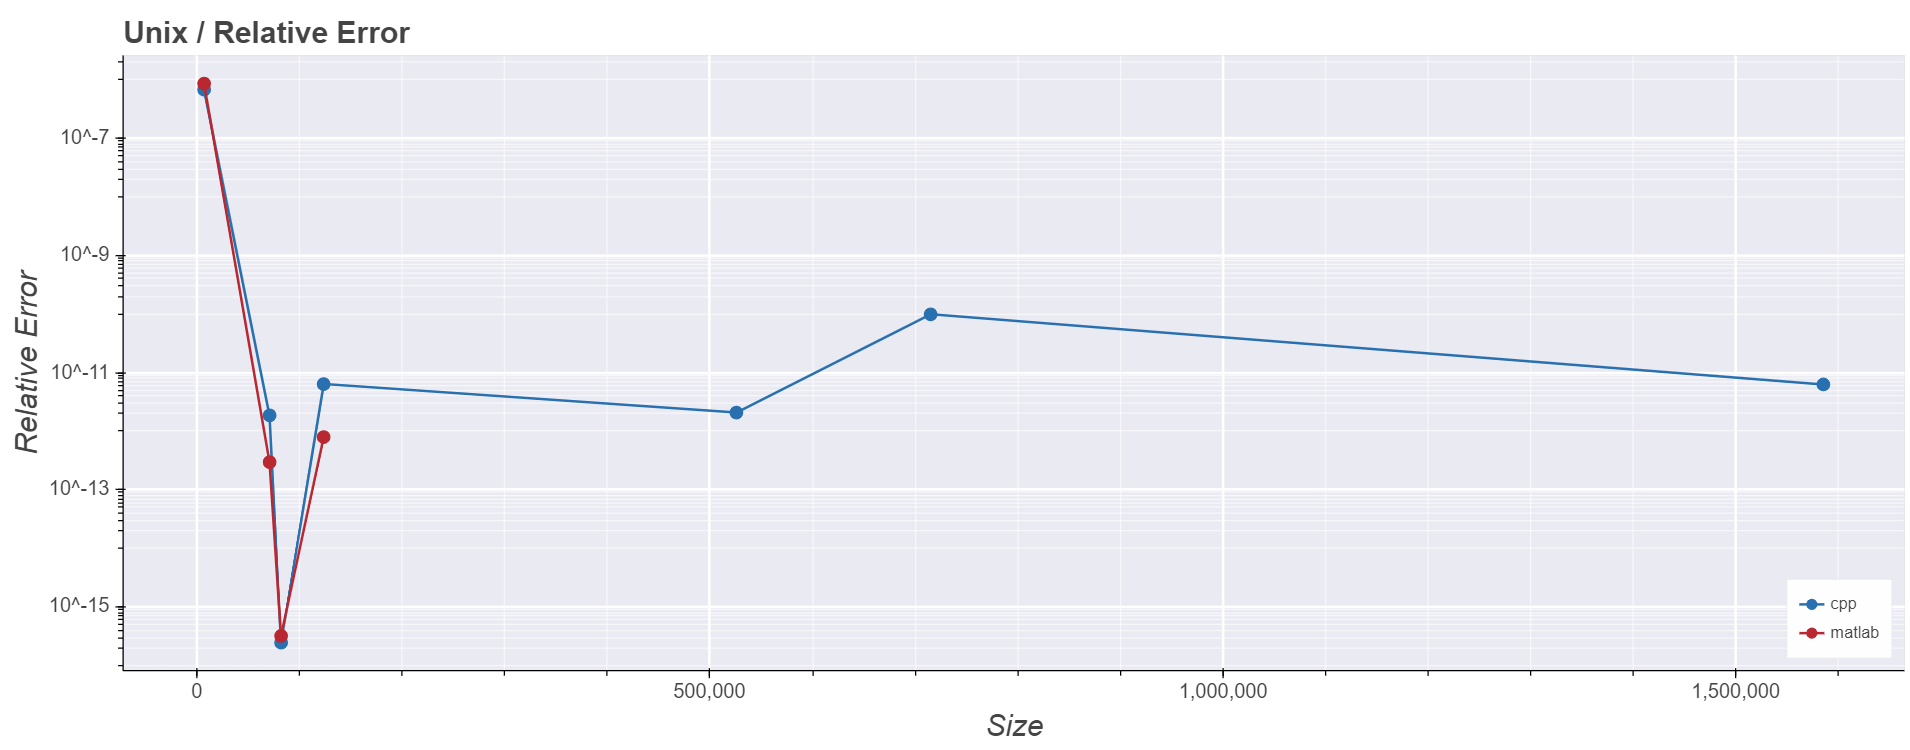
\includegraphics[width=1.3\linewidth]{unix_error.png}}
    \caption{Errore relativo su Linux}
    \label{fig:linux-error}
\end{figure}

\newpage
\section{Risultati per implementazione}
\label{section-results-os}

\subsection{C++}
\subsubsection*{Tempo}
Come illustrato in \cref{fig:cpp-time}, Linux risulta più efficiente di Windows nell'esecuzione dell'implementazione C++ per tutte le matrici analizzate.
\begin{figure}[H]
    \makebox[\textwidth][c]{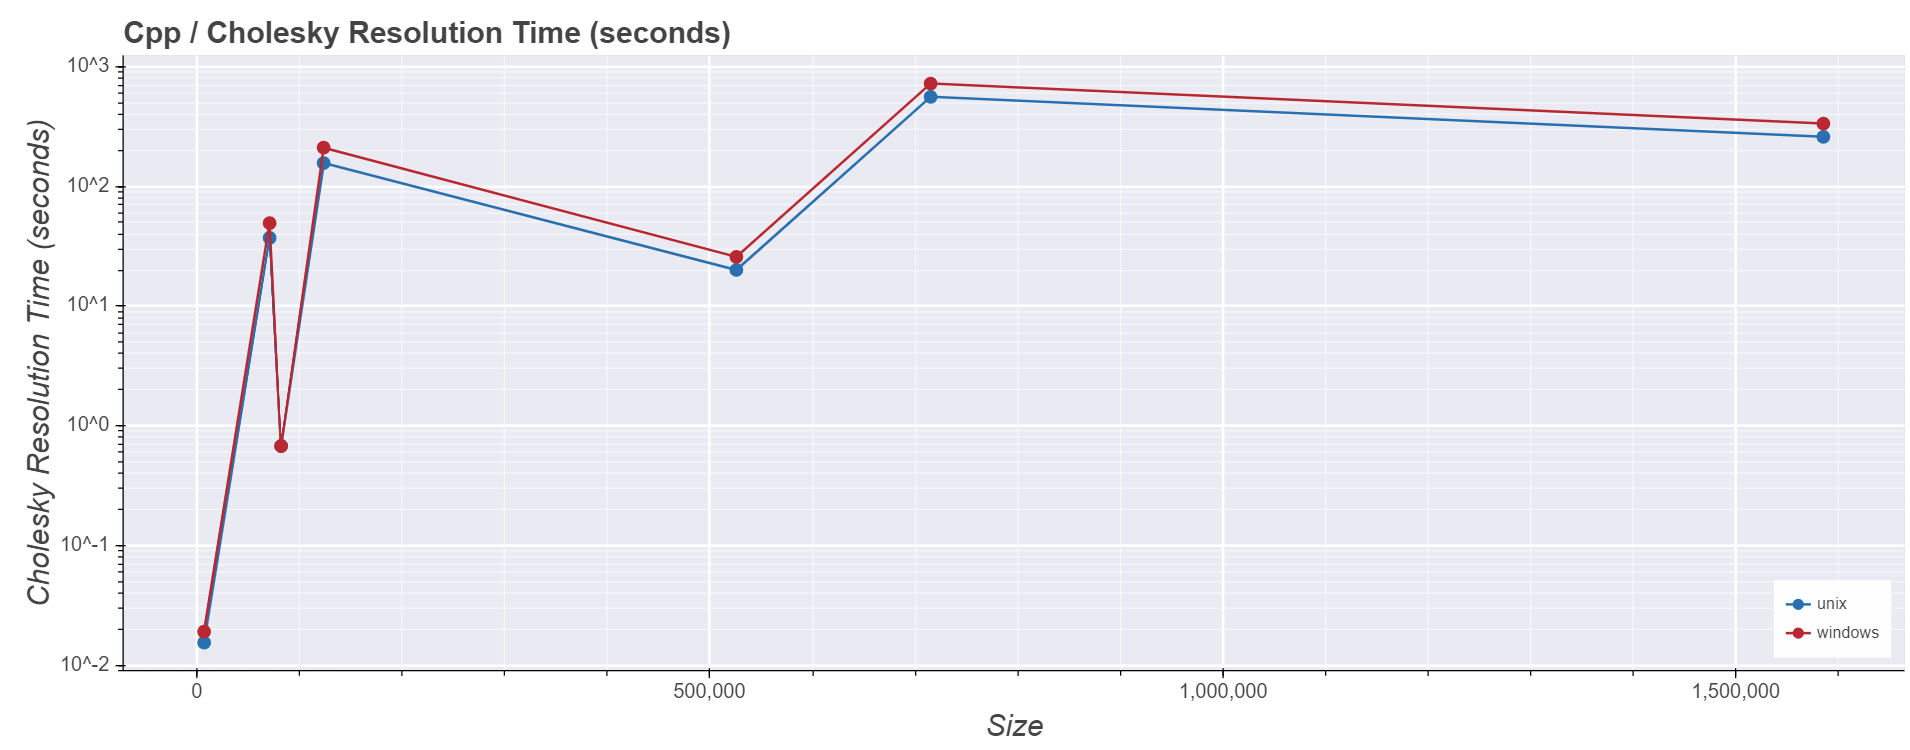
\includegraphics[width=1.18\linewidth]{cpp_solve.png}}
    \caption{Tempo di risoluzione nell'implementazione C++}
    \label{fig:cpp-time}
\end{figure}

\subsubsection*{Errore Relativo}
L'errore relativo non risulta influenzato dal diverso ambiente sul quale viene eseguita l'implementazione.
\begin{figure}[H]
    \makebox[\textwidth][c]{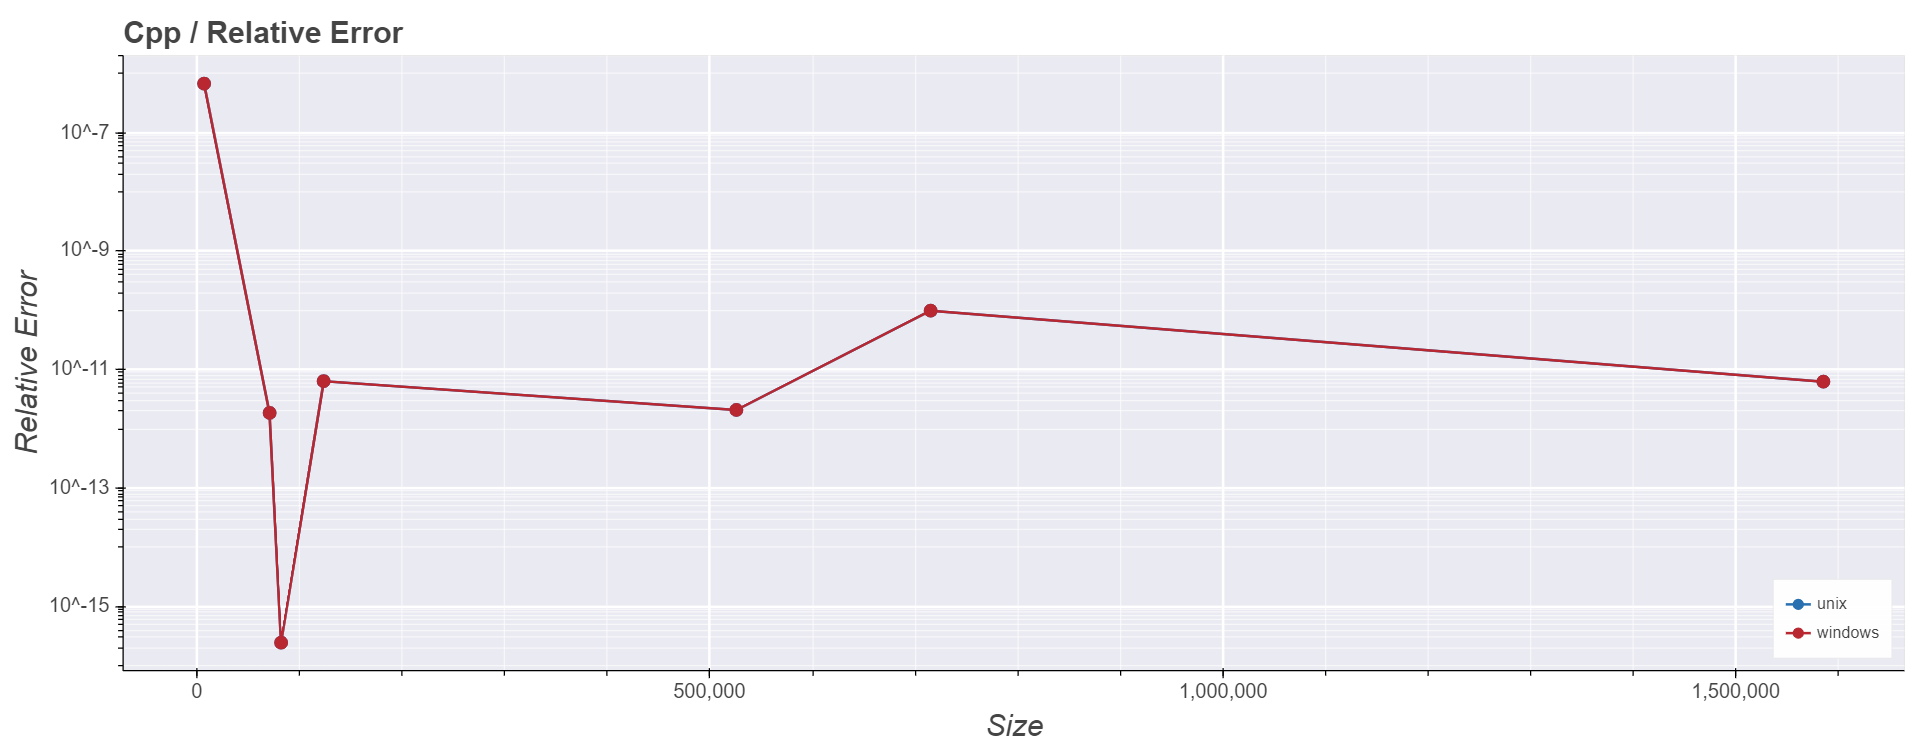
\includegraphics[width=1.18\linewidth]{cpp_error.png}}
    \caption{Errore relativo nell'implementazione C++}
    \label{fig:cpp-error}
\end{figure}

\subsubsection*{Memoria}
Al crescere della dimensione della matrice, la memoria impiegata per la risoluzione tende ad essere pressoché identica nei due ambienti.
\begin{figure}[H]
    \makebox[\textwidth][c]{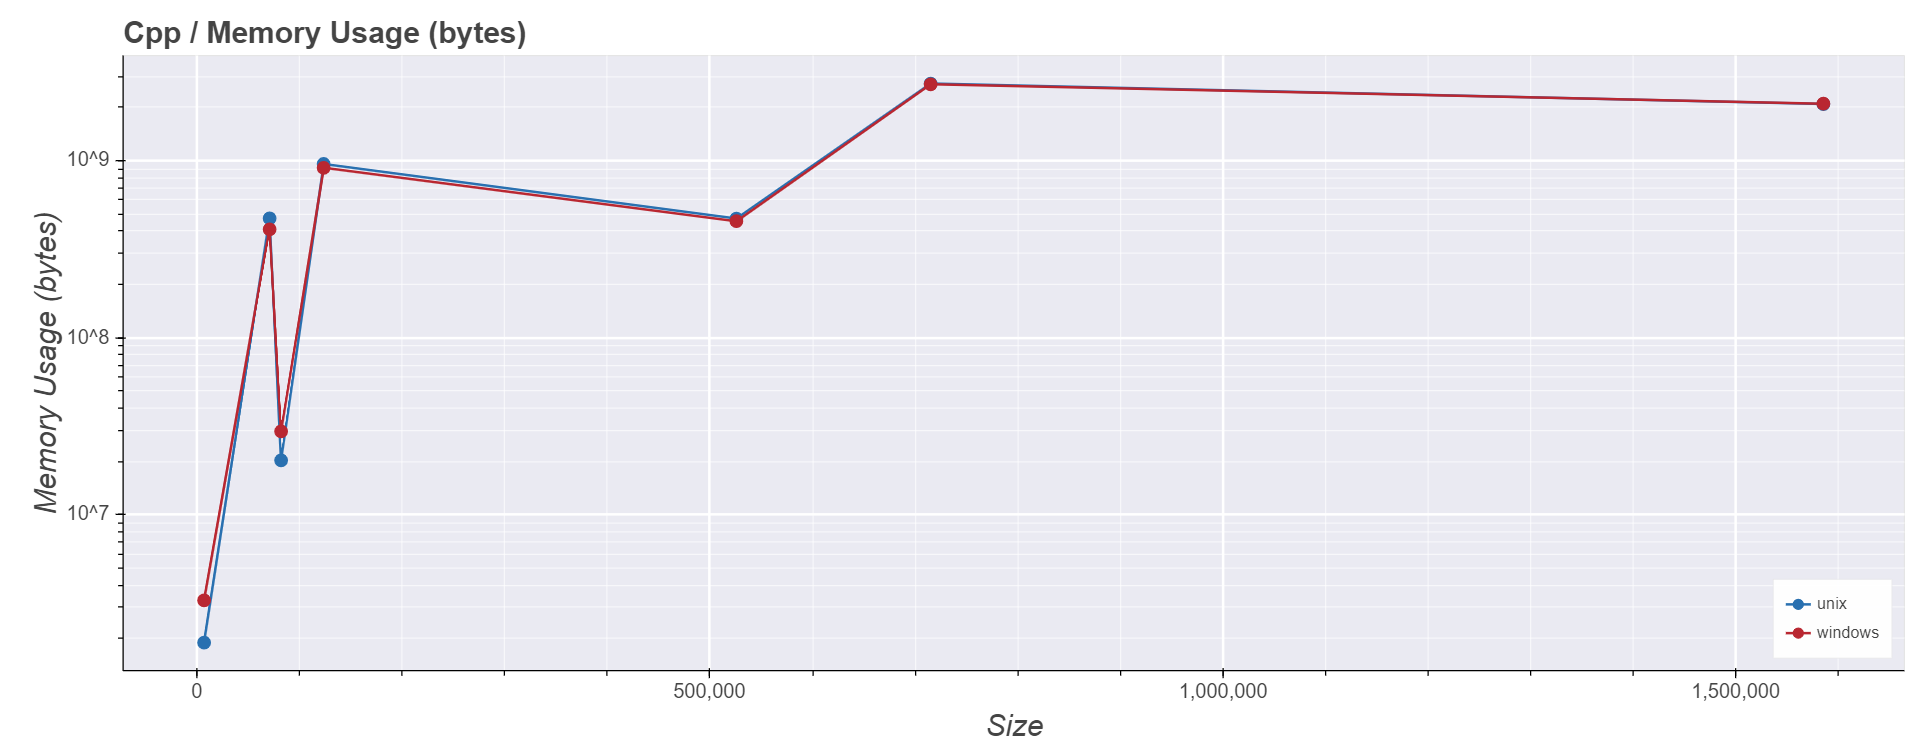
\includegraphics[width=1.2\linewidth]{cpp_memory.png}}
    \caption{Utilizzo della memoria nell'implementazione C++}
    \label{fig:cpp-memory}
\end{figure}

\subsection{Matlab}
\subsubsection*{Tempo}
L'esecuzione dello script MATLAB in ambiente Linux risulta essere più efficiente. In questo caso, la differenza risulta ancora più marcata rispetto all'implementazione C++ illustrata in \cref{fig:cpp-time}.
\begin{figure}[H]
    \makebox[\textwidth][c]{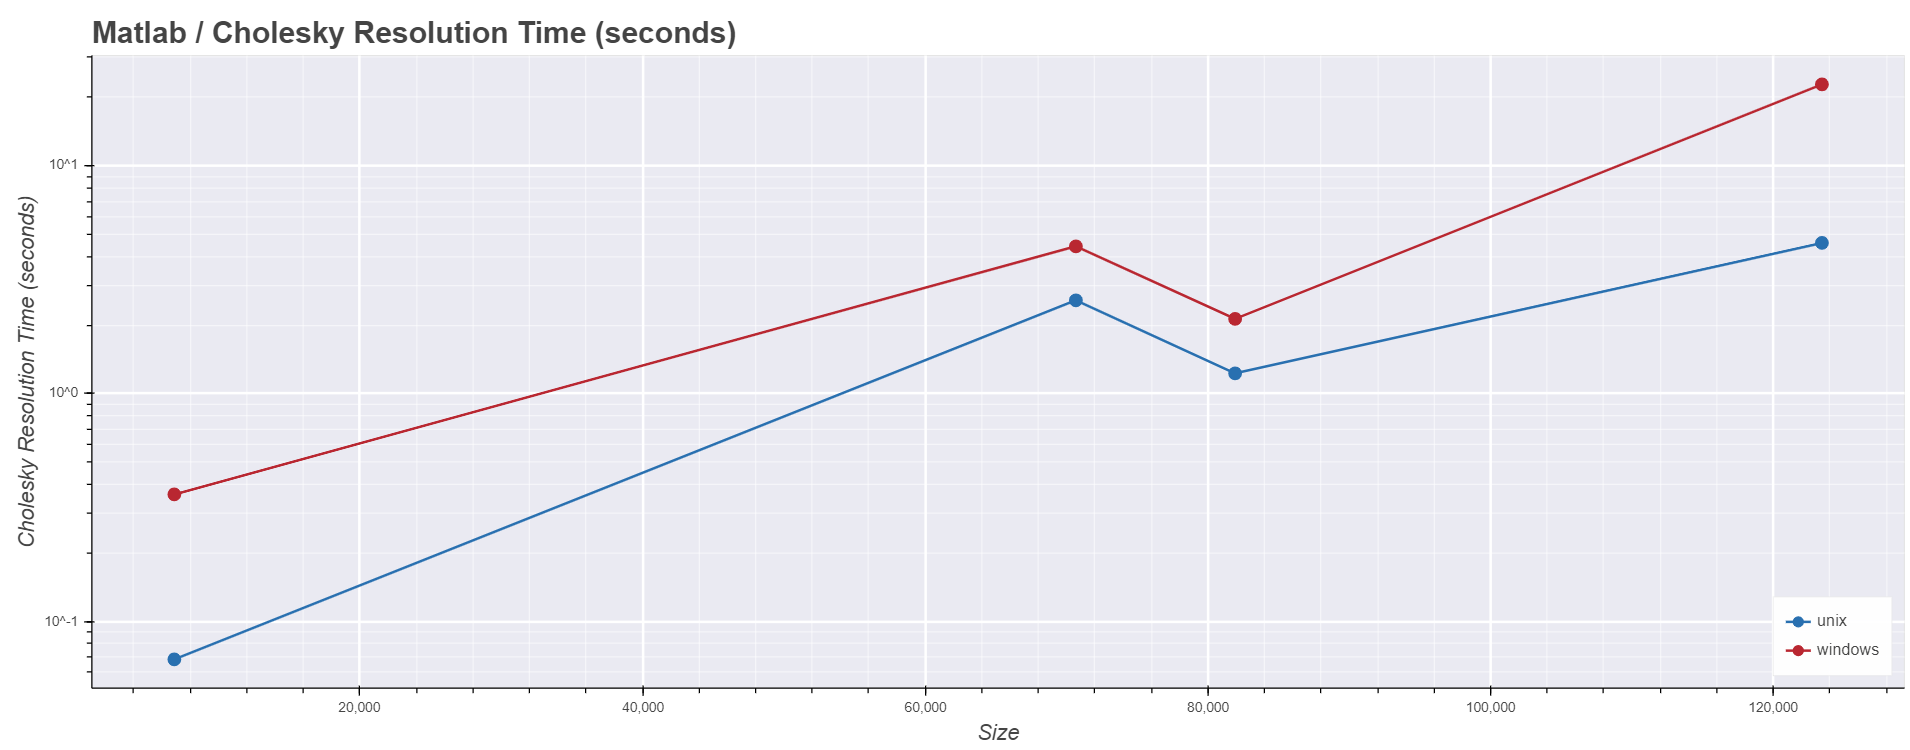
\includegraphics[width=1.2\linewidth]{matlab_solve.png}}
    \caption{Tempo di risoluzione nell'implementazione MATLAB}
    \label{fig:matlab-time}
\end{figure}

\subsubsection*{Errore Relativo}
L'errore relativo dei risultati della libreria Matlab non cambia a seconda delle archittetture.
\begin{figure}[H]
    \makebox[\textwidth][c]{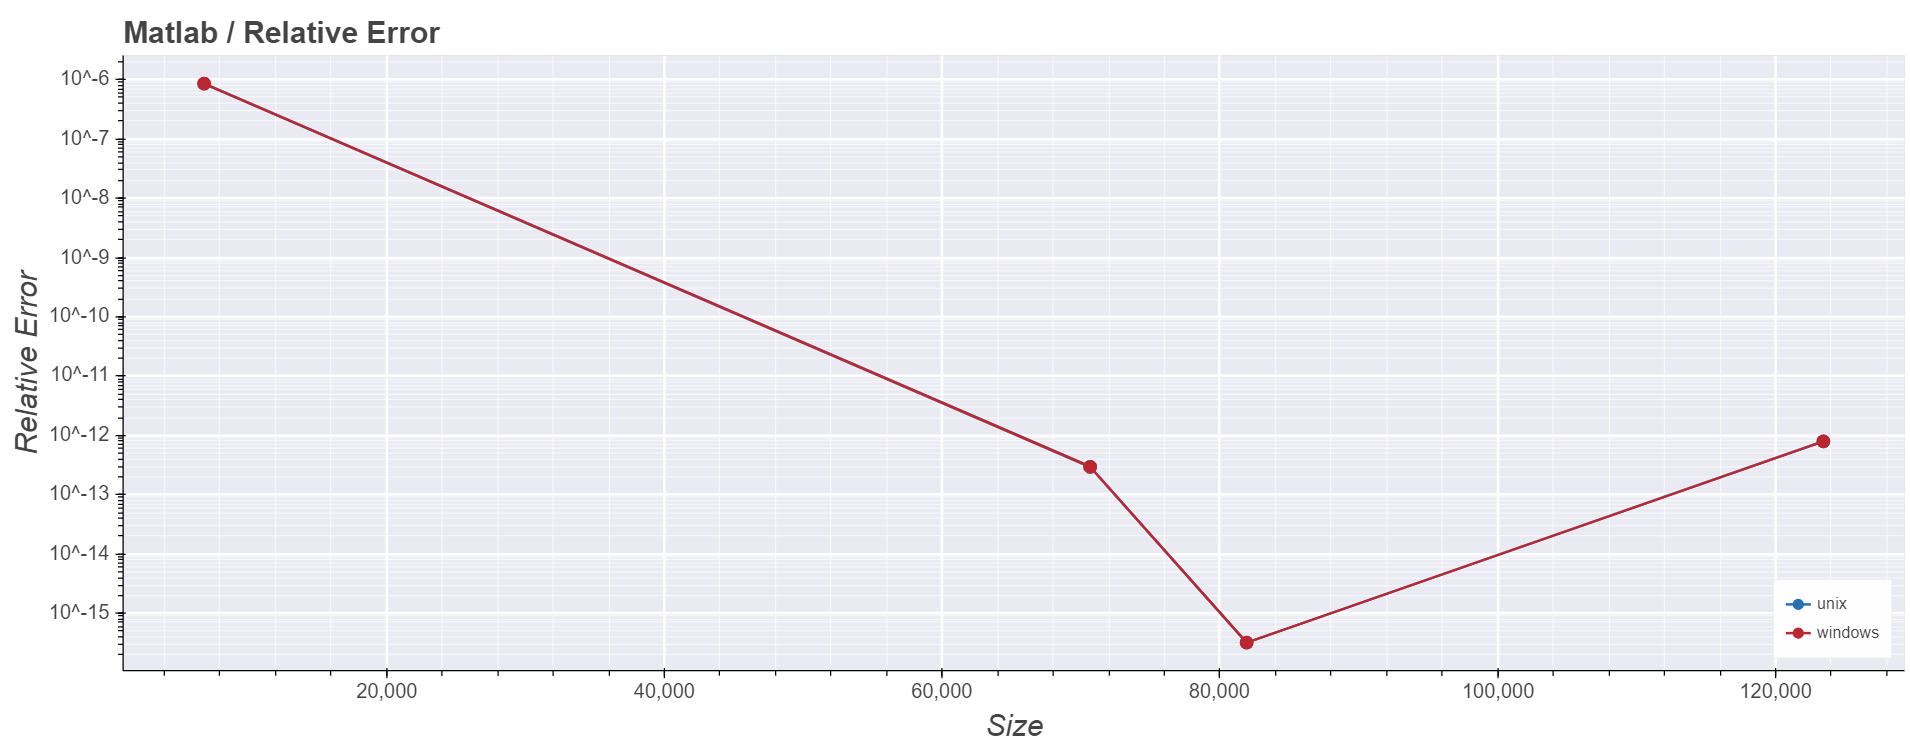
\includegraphics[width=1.3\linewidth]{matlab_error.png}}
    \caption{Errore relativo nell'implementazione MATLAB}
    \label{fig:matlab-error}
\end{figure}

\subsubsection*{Memoria}
La differenza di memoria utilizzata nelle due architetture è visibile solo sull'esecuzionen della prima matrice, le restanti impiegano pressoché lo stesso quantitativo di memoria.
\begin{figure}[H]
    \makebox[\textwidth][c]{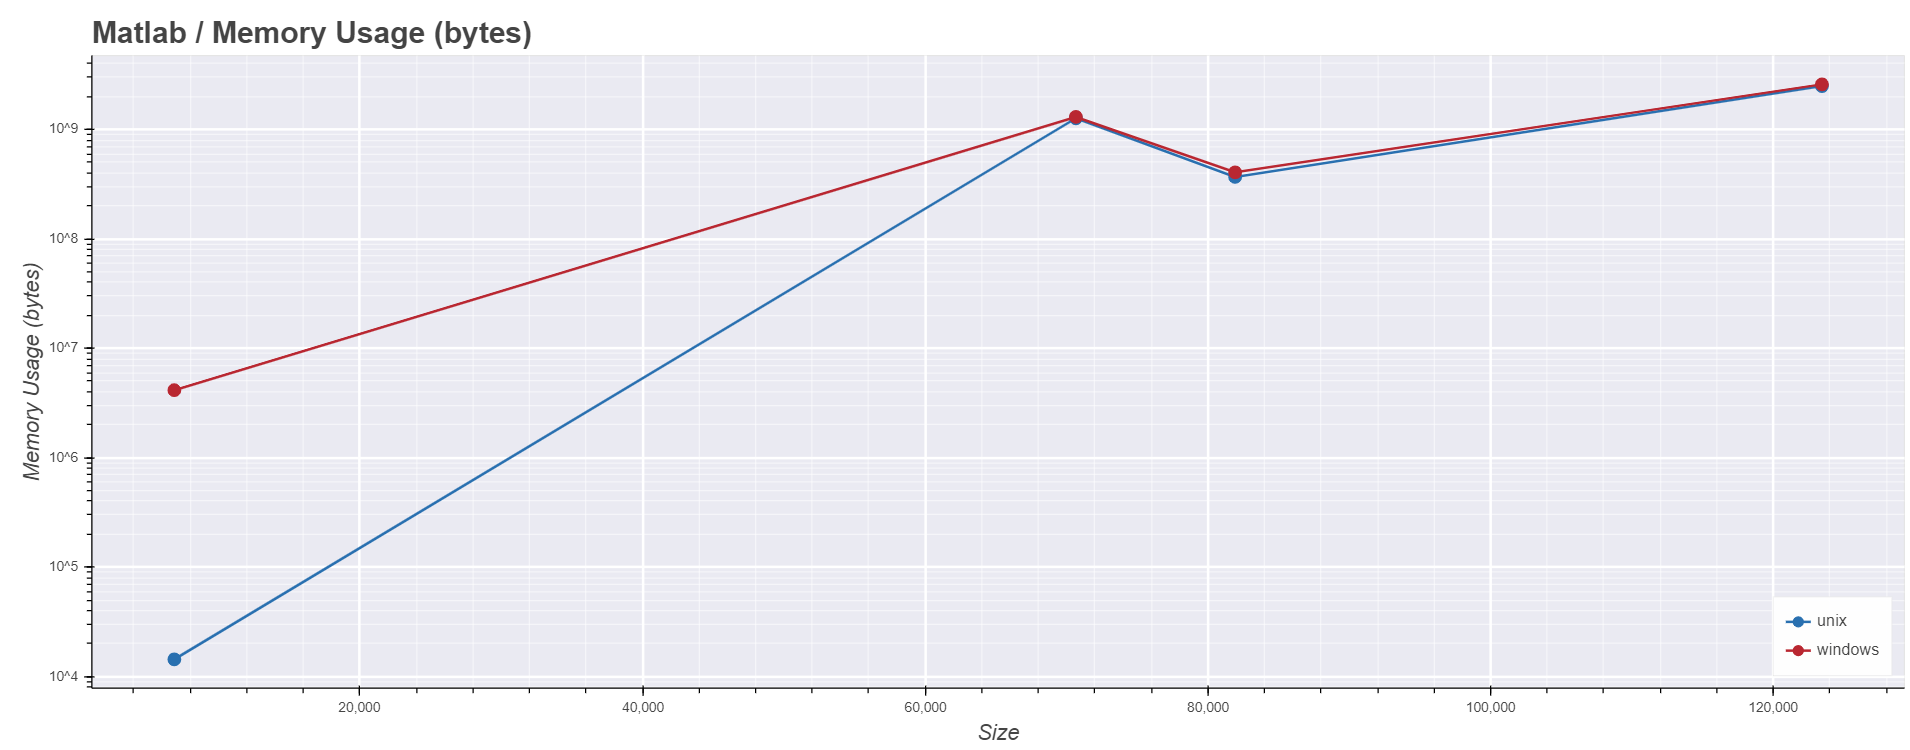
\includegraphics[width=1.3\linewidth]{matlab_memory.png}}
    \caption{Utilizzo della memoria nell'implementazione MATLAB}
    \label{fig:matlab-memory}
\end{figure}

\newpage
\section{Conclusioni}
Dai risultati ottenuti, il problema principale di MATLAB risulta l'eccessivo utilizzo di memoria RAM. Al contrario, C++ riesce a risolvere matrici di dimensioni più grandi grazie ad una gestione più efficiente ed un minor overhead del linguaggio.

\smallskip
Analizzando i tempi di esecuzione invece, la situazione si ribalta. MATLAB riesce a ridurre notevolmente i tempi di attesa per la soluzione del sistema soprattutto al crescere della dimensione della matrice.
Invece, C++ impiega un tempo maggiore nell'ordine di alcuni minuti (comparabile solo sulle matrici per le quali si è riusciti ad avere una soluzione in entrambe le implementazioni).

Questa differenza così marcata è spiegabile facilmente: MATLAB è un software che esegue calcoli in parallelo e sfrutta tutti i core presenti sulla sistema utilizzato, inoltre le operazioni più comuni in ambito matematico ci si aspetta che siano ottimizzate a dovere.
D'altro canto, l'implementazione C++ al momento è un processo single core, non riuscendo quindi a sfruttare la totale potenza del processore ed impiegando più tempo.

Questa ipotesi è rafforzata dal confronto tra \cref{fig:cpp-time,fig:linux-time}, infatti MATLAB riesce a beneficiare dell'esecuzione multicore rimarcando ancora di più la differenza nei tempi di esecuzione rispetto a C++.

\smallskip
Analizzando le due implementazioni sui diversi sistemi operativi possiamo affermare con sicurezza che Linux riesca ad eseguire in modo più prestante le due implementazioni.

\smallskip
In conclusione, i risultati mostrano come la libreria Eigen per C++ prediliga un utilizzo più efficiente della memoria, penalizzando il tempo di esecuzione. Questo, a parità di hardware, permette di lavorare su matrici di dimensioni maggiori a discapito di un codice più complesso e meno intuitivo.

\newpage
\section{Listati di codice}
\label{section:code}
\begin{lstlisting}[language=C++,emph={std},basicstyle=\footnotesize\ttfamily,caption=Main dell'implementazione C++]
int main() {
    result _result;
    std::ofstream output(OUTPUT_FILE, std::ofstream::out);

    // Write headers
    output << "filename" << ","
        << "size" << ","
        << "memory_delta" << ","
        << "solve_time" << ","
        << "relative_error" << CSV_EOL;

    // Look for matrix in ../matlab/matrix_mtx folder
    std::string path = "../matlab/matrix_mtx";
    for (const auto& entry : std::filesystem::directory_iterator(path)) {
        if (entry.path().extension() == ".mtx") {
            if (! output.is_open()) {
                output.open(OUTPUT_FILE, std::ofstream::app);
            }

            std::cout << entry.path() << std::endl;
            _result = analyze_matrix(entry.path().string());

            output << entry.path().stem() << "," << _result << CSV_EOL;
            output.close();
        }
    }

    return 0;
}
\end{lstlisting}

\newpage
\begin{lstlisting}[language=C++,basicstyle=\footnotesize\ttfamily,caption=Lettura della memoria in C++]
// Adapted from: https://stackoverflow.com/questions/63166/how-to-determine-cpu-and-memory-consumption-from-inside-a-process
unsigned long long memory::process_current_physical() {
#ifdef OS_WIN
    PROCESS_MEMORY_COUNTERS_EX pmc;
    GetProcessMemoryInfo(GetCurrentProcess(), (PROCESS_MEMORY_COUNTERS*)&pmc, sizeof(pmc));

    return pmc.WorkingSetSize;
#elif defined(OS_NIX)
    long rss = 0L;
    FILE* fp = NULL;

    if ((fp = fopen("/proc/self/statm", "r")) == NULL) {
        return (size_t)0L;
    }

    if (fscanf(fp, "%*s%ld", &rss) != 1) {
        fclose(fp);
        return (size_t) 0L;
    }

    fclose(fp);
    return (size_t) rss * (size_t) sysconf(_SC_PAGESIZE);
#endif
}
\end{lstlisting}

\newpage
\begin{lstlisting}[language=MatLab,basicstyle=\footnotesize\ttfamily,caption=Main dell'implementazione MATLAB]
path = fullfile('matrix_mat', '*.mat');
files = dir(path);
filesCount = length(files);

results = ["filename", "size", "memory_delta", "solve_time", "relative_error"];

for K = 1 : filesCount
  filename = convertCharsToStrings(files(K).name);
  [size, memory_delta, solve_time, relative_error] = chol_solve(filename, 1);

  results = [results(1:K,:); [strtok(filename, '.'),size,memory_delta,solve_time,relative_error]];
  clearvars filename size memory_delta solve_time relative_error;
end

if isunix
  writematrix(results, 'unix-output.csv');
elseif ispc
  writematrix(results, 'windows-output.csv');
end
\end{lstlisting}

\newpage
\begin{lstlisting}[language=MatLab,basicstyle=\footnotesize\ttfamily,caption=Funzione di conversione da \lstinline{.mat} a \lstinline{.mtx} per matrici simmetriche]
function [ err ] = mmwrite_symmetric(filename,A)
mattype = 'real';
precision = 16;
comment = '';

mmfile = fopen([filename],'w');
if (mmfile == -1)
  error('Cannot open file for output');
end;

[M,N] = size(A);
if (issparse(A))
  [I,J,V] = find(A);

  issymm = 0;
  symm = 'general';
  [I,J,V] = find(A);
  NZ = nnz(A);

  rep = 'coordinate';

  fprintf(mmfile, '%%%%MatrixMarket matrix %s %s %s\n', 'coordinate', mattype, symm);

  [MC,NC] = size(comment);
  if (MC == 0)
    fprintf(mmfile, '%% Generated %s\n', [date]);
  else
    for i = 1:MC,
      fprintf(mmfile, '%%%s\n', comment(i, :));
    end
  end

  fprintf(mmfile, '%d %d %d\n', M, N, NZ);
  realformat = sprintf('%%d %%d %% .%dg\n', precision);

  for i = 1:NZ
    fprintf(mmfile, realformat, I(i), J(i), V(i));
  end;
end
fclose(mmfile);
\end{lstlisting}
\end{document}